\section{Invention of my favourite gadgets}
I told in previous section that computer and smart phone are my favourite gadgets. A computer is a digital electronic machine that can be programmed to carry out sequences of arithmetic or logical operations (computation) automatically. On the other hand a mobile phone is a wireless handheld device that 
\begin{table}[h]
    \centering
    \begin{tabular}{|c|c|c|}
    \hline
     Invention & Inventor & year  \\
     \hline
    Telephone phone &  Alexander Graham Bell & 1876\\
    \hline
    Computer & Charles Babbage & 1822\\
    \hline
    \end{tabular}
    \caption{Invention of favourite gadgets}
    \label{tab:my_label}
\end{table}\\
 allows users to make and receive calls. In table~\ref{tab:my_label}, I have shown the invention, inventor and invention year of my favourite gadgets. Here I discuss about the invention of computer and mobile phone.
\subsection{Invention of computer}
In~\cite{slater1987invented}, slater1987invented et al., proved that John Vincent Attanasoff beleived that he was the inventor of computer. The computer name was the Atanasoff–Berry computer (ABC). The machine Attanasoff built from 1939 to 1942 used 300 vacuum tubes for the logic circuitry and capacitors for automatic "jogging" or regeneration of memory. It was the first machine to perform arithmetic electronically. 
\begin{figure}[h]
    \centering
    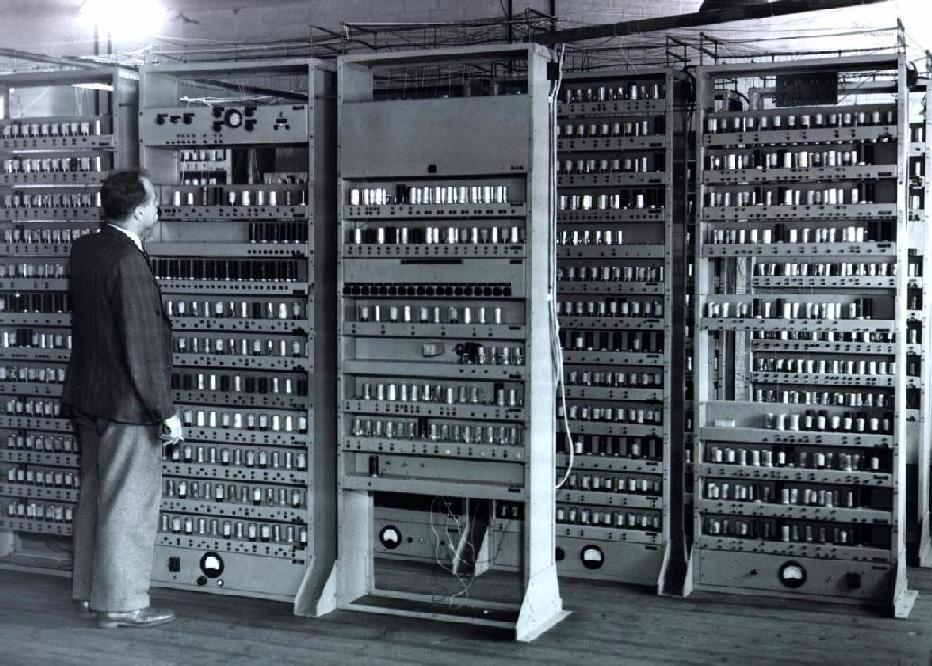
\includegraphics[width = 0.8\textwidth]{pic/first_computer.jpeg}
    \caption{World first computer}
    \label{fig:fig4}
\end{figure}\\
In figure~\ref{fig:fig4}, I have shown the first computer of the world. Before ABC, there were mechanical computing devices that could perform simple calculations. The first mechanical computer, The Babbage Difference Engine, was designed by Charles Babbage in 1822. The ABC was the basis for the modern computer we all use today.
\subsection{Invention of mobile phone}
In~\cite{agar2013constant}, agar2013constant et al., provided that  Alexander Graham Bell invented the telephone in 1876. And then in 1900, on December 23 on the outskirts of Washington, D.C., an inventor named Reginald Fessenden accomplished a remarkable feat. He made the first wireless telephone call. He was the first to transmit the human voice via radio waves, sending a signal from one radio tower to another.
\begin{figure}[h]
    \centering
    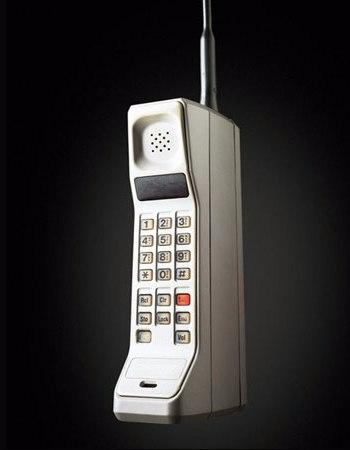
\includegraphics[width = 0.5\textwidth]{pic/first_cellphone.jpeg}
    \caption{Wireless telephone}
    \label{fig:fig5}
\end{figure}\\
The telephone of that era was large in size. Gradually with time passed, the size of telephone reduced and became use as a wireless device. \\1G mobile communication system was introduced in Japan in 1979 by Nippon Telegraph and Telephone (NTT). Initially, it started in Tokyo and within next five years expanded to cover the whole of Japan.\\
In 1981, Nordic Mobile Telephone (NMT) was launched in European countries. In 1983, Ameritech launched 1G mobiles in the USA using Motorola mobile phones. Use of mobile communication system was then followed by several countries\\
Gradually more and more researches were done in the device and new generation of mobile phons wire made.
